Deux signaux peuvent être déphasés, c'est à dire décalés.
	
	\textbf{Déphasage de 180\degre} : on parle aussi d'opposition de phase. La courbe rouge est décalée de $\pi$ (équation : $y=sin(x)$) par rapport à la courbe noire (équation : $y=sin(x+\pi)$).
	
	\begin{figure}[H]
	\begin{center}
	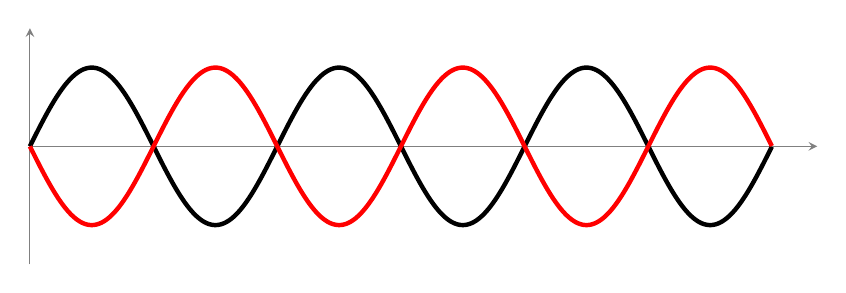
\begin{tikzpicture}[scale=0.5,samples=500]
	\draw[color=gray,thin,->,>=stealth] (0,0)--(20,0); % l'axe des abscisses
	\draw[color=gray,thin,->,>=stealth] (0,-3)--(0,3); % l'axe des ordonnées
	\draw [ultra thick,domain=0:6*pi] plot (\x,{2*sin(\x r)});
	\draw [color=red,ultra thick,domain=0:6*pi] plot (\x,{2*sin((\x+pi) r)});
	\end{tikzpicture}
	\end{center}
	\caption{Déphasage de 180\degre}
	\end{figure}
	
	\textbf{Déphasage de 90\degre} : même principe, mais on ne décale cette fois que de $\dfrac{\pi}{2}$, les 2 équations sont respectivement $y=sin(x)$ et $y=sin(x+\dfrac{\pi}{2})$.
	
	\begin{figure}[H]
	\begin{center}
	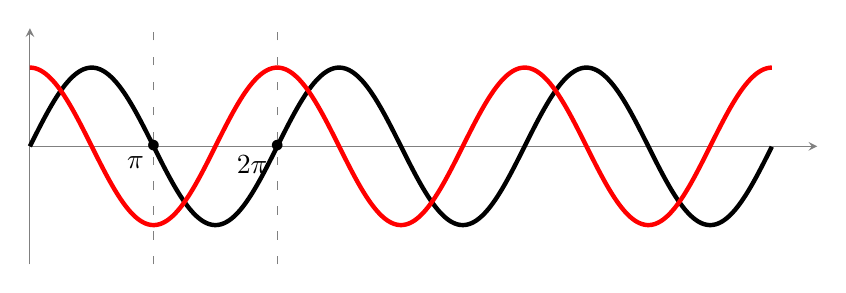
\begin{tikzpicture}[scale=0.5,samples=500]
	\draw[color=gray,thin,->,>=stealth] (0,0)--(20,0); % l'axe des abscisses
	\draw[color=gray,thin,->,>=stealth] (0,-3)--(0,3); % l'axe des ordonnées
	\draw[color=gray,loosely dashed] (pi,-3)--(pi,3);
	\draw[color=gray,loosely dashed] (2*pi,-3)--(2*pi,3);
	\draw [ultra thick,domain=0:6*pi] plot (\x,{2*sin(\x r)});
	\draw [color=red,ultra thick,domain=0:6*pi] plot (\x,{2*sin((\x+pi/2) r)});
	
	\draw (pi,0) node[below left] {$\pi$} node{$\bullet$};
	\draw (2*pi,0) node[below left] {$2\pi$} node{$\bullet$};
	\end{tikzpicture}
	\end{center}
	\caption{Déphasage de 90\degre}
	\end{figure}
	
	\textbf{Déphasage de 45\degre} : toujours le même principe, mais on ne décale cette fois que de $\dfrac{\pi}{4}$, les 2 équations sont respectivement $y=sin(x)$ et $y=sin(x+\dfrac{\pi}{4})$.
	
	\begin{figure}[H]
	\begin{center}
	\begin{tikzpicture}[scale=0.5,samples=500]
	\draw[color=gray,thin,->,>=stealth] (0,0)--(20,0); % l'axe des abscisses
	\draw[color=gray,thin,->,>=stealth] (0,-3)--(0,3); % l'axe des ordonnées
	\draw[color=gray,loosely dashed] (pi,-3)--(pi,3);
	\draw[color=gray,loosely dashed] (2*pi,-3)--(2*pi,3);
	\draw[color=gray,loosely dashed] (0,2*0.707)--(2*pi,2*0.707);
	\draw[color=gray,loosely dashed] (0,-2*0.707)--(pi,-2*0.707);
	
	\draw [ultra thick,domain=0:6*pi] plot (\x,{2*sin(\x r)});
	\draw [color=red,ultra thick,domain=0:6*pi] plot (\x,{2*sin((\x+pi/4) r)});
	
	\draw (pi,0) node[below left] {$\pi$} node{$\bullet$};
	\draw (2*pi,0) node[below left] {$2\pi$} node{$\bullet$};
	\draw (0,2*0.707) node[left,scale=0.5] {$\cos\left(\dfrac{\pi}{4}\right) \simeq 0.707 $};
	\draw (0,-2*0.707) node[left,scale=0.5] {$-\cos\left(\dfrac{\pi}{4}\right) \simeq -0.707 $};
	\end{tikzpicture}
	\end{center}
	\caption{Déphasage de 45\degre}
	\end{figure}
